\documentclass[11pt]{amsart}
\usepackage[utf8]{inputenc}
\usepackage{amsmath, amssymb}
\usepackage{color}
\usepackage{tkz-euclide}
\usetikzlibrary{patterns, intersections}

\begin{document}

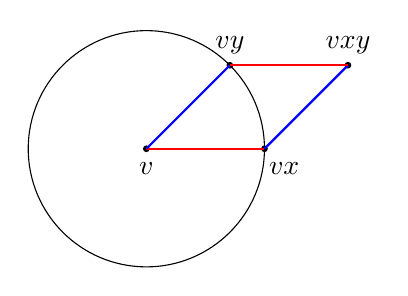
\begin{tikzpicture}
\draw (0,0) circle (1.5cm);

\filldraw (0,0) circle (0.035) node[yshift=-.25cm] {$v$}
(1.5,0) circle (0.035) node[yshift=-.25cm ,xshift=.25cm] {$vx$};

\begin{scope}[rotate=45]
\filldraw (1.5,0) circle (0.035) node[yshift=.25 cm] {$vy$};

\begin{scope}[shift={(1.5,0)},rotate=45]
\filldraw (0,-1.5) circle (0.035) node[yshift=.25cm] {$vxy$};
\end{scope}
\end{scope}

\draw[thick,red] (0,0) -- (1.5,0);

\begin{scope}[rotate=45]
\draw[thick,blue] (0,0) -- (1.5,0);
\end{scope}

\begin{scope}[shift={(1.5,0)},rotate=45]
\draw[thick,blue] (0,0) -- (1.5,0);
\end{scope}

\begin{scope}[shift={({1.5*cos(45)},{(1.5*cos(45))})}]
\draw[thick,red] (0,0) -- (1.5,0);
\end{scope}
\end{tikzpicture}

\end{document}